% Activate the following line by filling in the right side. If for example the name of the root file is Main.tex, write
% "...root = Main.tex" if the chapter file is in the same directory, and "...root = ../Main.tex" if the chapter is in a subdirectory.
 
%!TEX root =  ../plantillaTFG.tex 
%recuerda que si cambias el nombre del fichero... debes cambiarlo aqui
\chapter{Introduction}
%\normalfont
 
\section{Semantic segmentation}
%\lettrine[lines=3]{\color{sepia}E}{}
In recent years, convolutional neural networks (CNNs) have become one of the most widely used machine learning techniques for the researchers in the field of computer vision. Many extensive applications of these models have come up within the rise of different CNN-based architectures, including medical image analysis (detection of diseases from CT or MR images), facial recognition (identify and verify the individuals in the images), object detection (detection of a specific object in the images or videos) and the very trending image fusion and generation using advanced architectures such as diffusion models.\\ 

Some of these applications can be grouped under a field known as semantic segmentation, which focuses on partitioning an image into multiple regions by classifying each pixel into a predefined category. For example, in medical imaging, some segmentation techniques have been used to perform identification of region-of-interest [1], like tumors, organs or other biological structures.\\ 

Another use of CNN model in the segmentation field is the land cover classification (Figure 1.1), which involves analyzing satellite or aerial images and labeling each pixel with classes such as water, forests, urban areas, agricultural lands, etc. These models are usually used for environmental monitoring to help track changes in natural habitats, deforestation rates, or water resource distribution over time [2].\\
\begin{figure}[h]
 \centering
 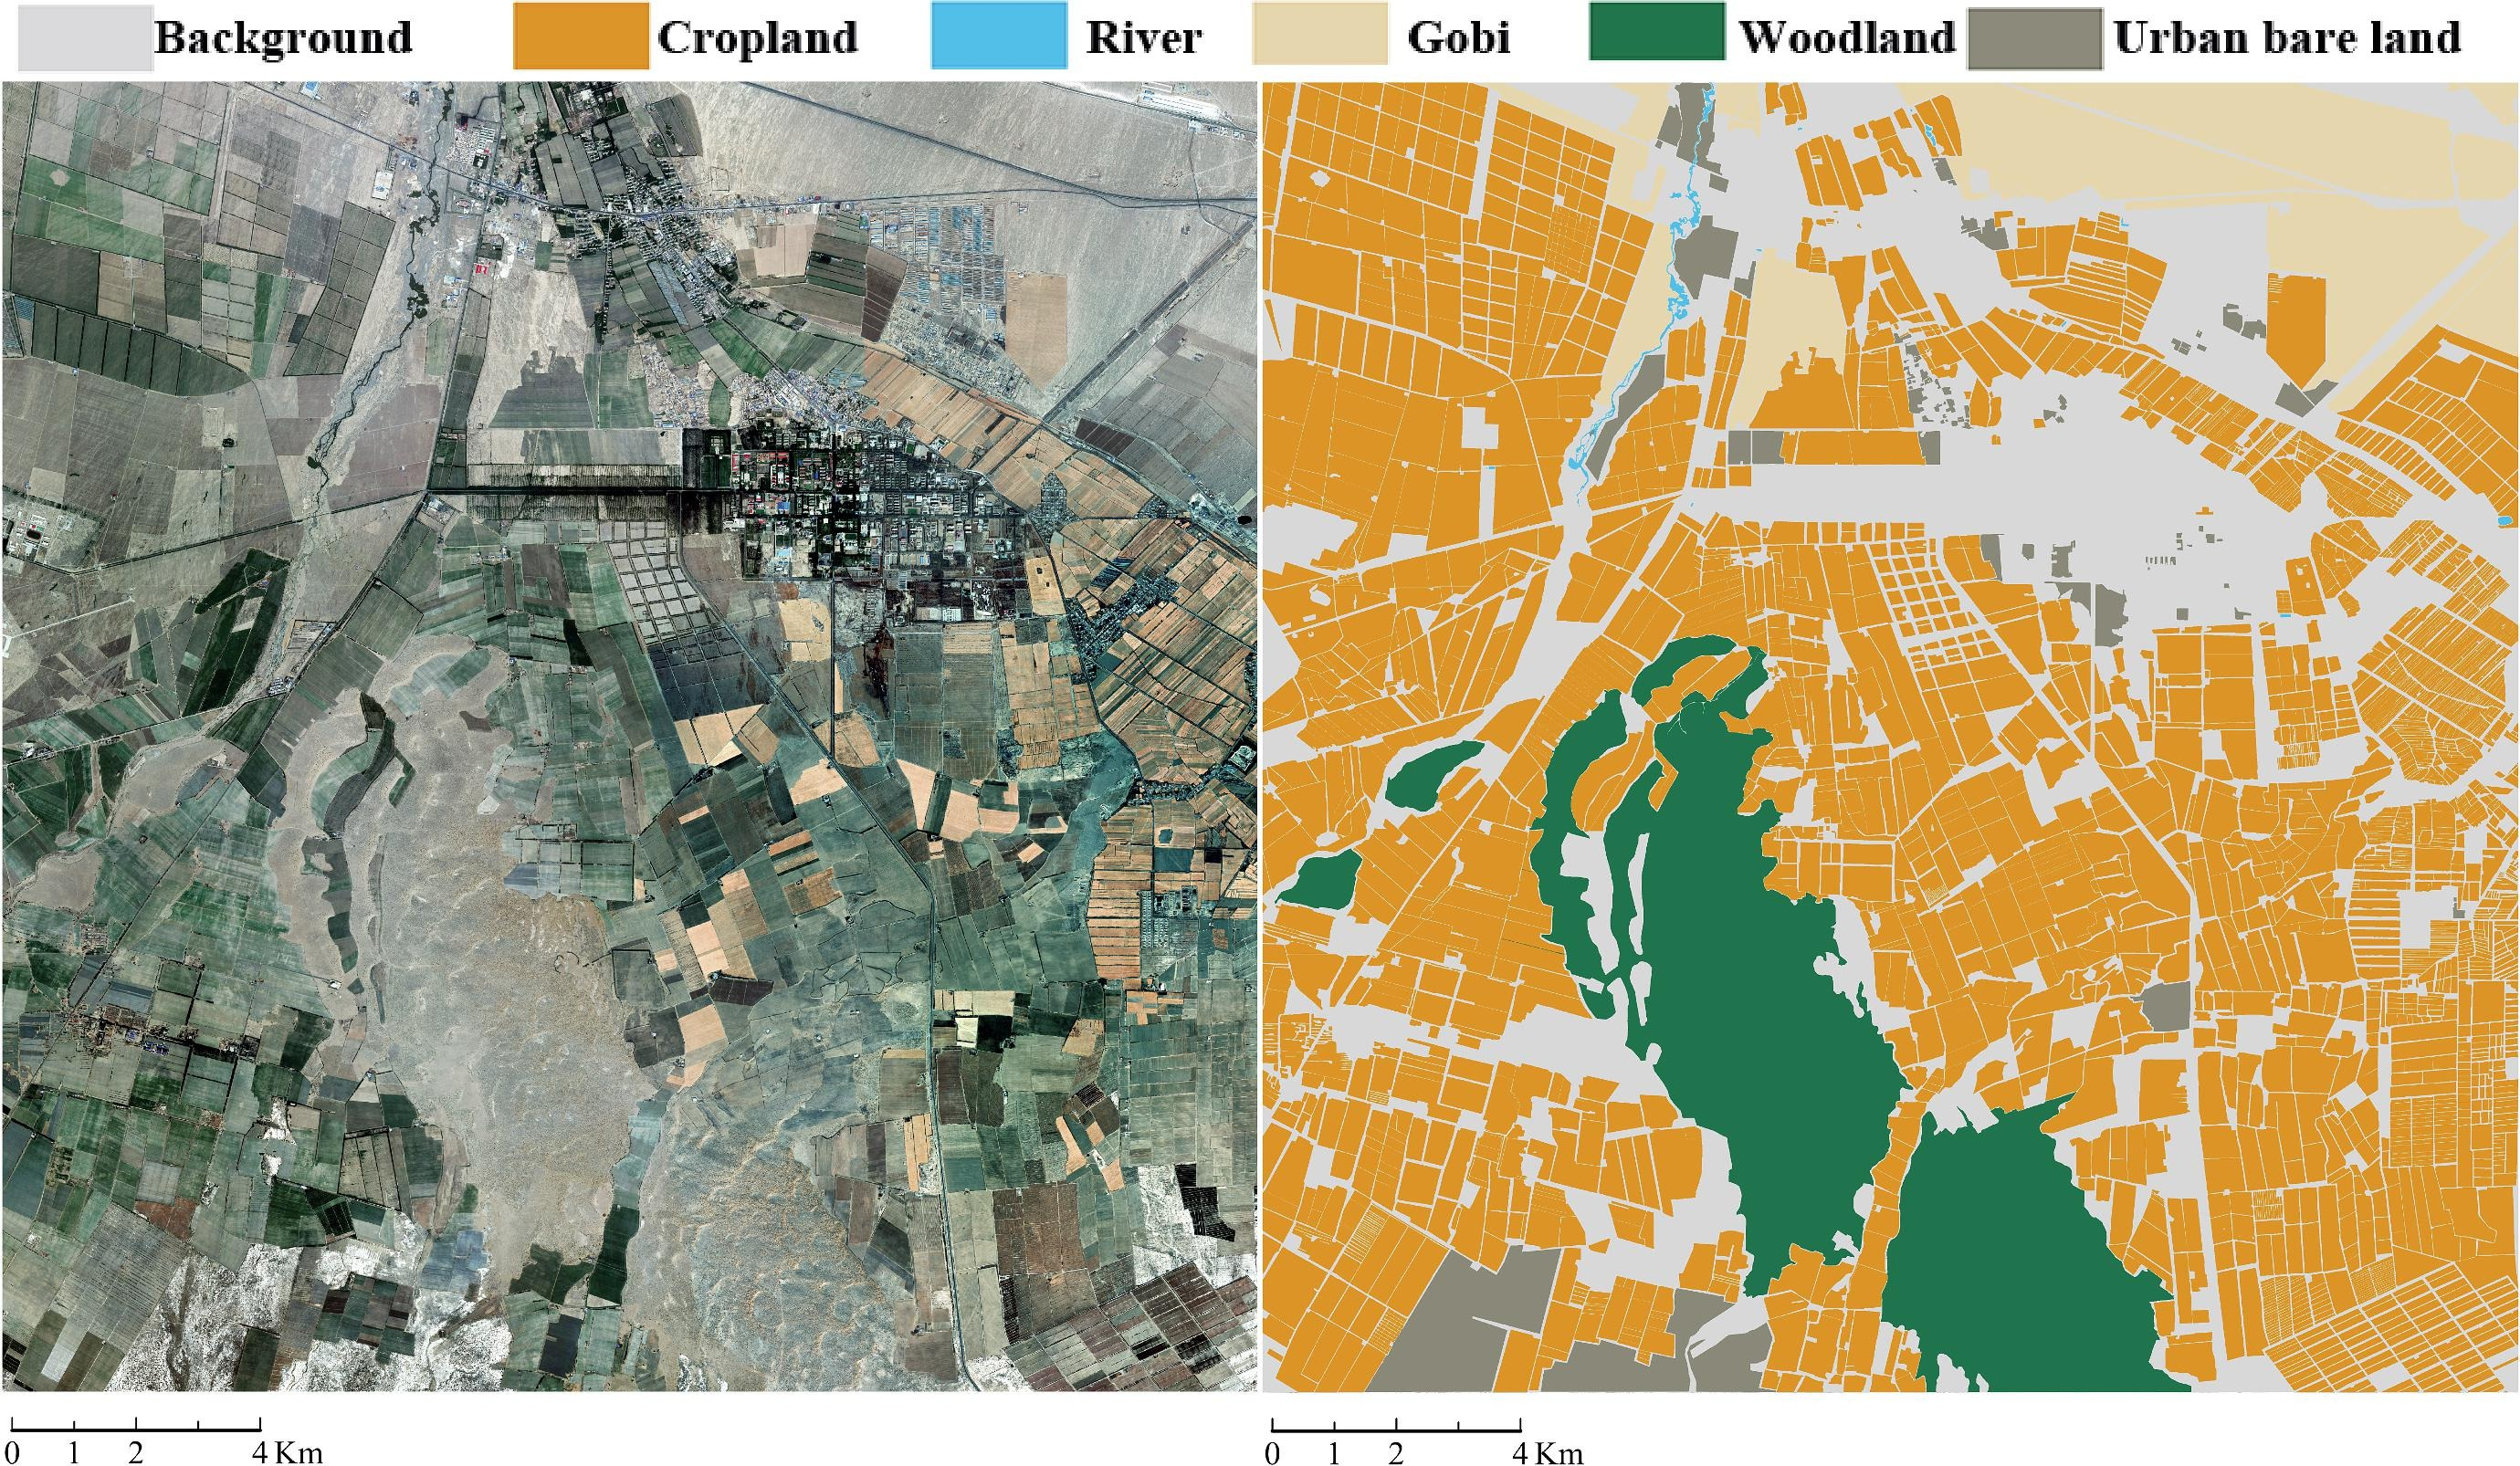
\includegraphics[scale=1.05]{IMAGENES/IMG1-Introduction.jpg}
 \captionsetup{font=large}
 \caption {Example of land cover segmentation. The left side shows the satellite image; the right side shows its ground truth mask. The image is segmented into six categories: Background, Cropland, River, Gobi, Woodland, and Urban bare land (image extracted from [1])}
\end{figure}


In this project, we focus on one specific subsection of land cover analysis: forest segmentation. The aim of the project is to monitor the spatial distribution and extent of forests in Cantabria, in order to detect changes and identify potential risks, such as the proximity of tree canopies to high-voltage power lines, which can result in severe incidents, including electrical short circuits, power outages, and even the ignition of wildfires. By using advanced image analysis and segmentation techniques, we will be able to map prediction mask on satellite imagery, assess their growth patterns, and identify risk zones where vegetation management is necessary. 

\newpage
\section{Motivation}
The project forms part of the internship at Alten-Worldgrid, a company that specializes in providing IT solutions to clients in the energy sector. For some of the clients, particularly those working with the operation and maintenance of electricity transmission networks, the potential contact between the tree canopies and high-voltage power lines has always been a major risk. There have been many reports [12,13] related to wildfires caused by the ignition of vegetation around utility poles. Such incidents may be triggered by overgrown tree canopies that come into contact with power lines or by extreme weather conditions that cause nearby trees to fall onto the lines.
\\


To prevent these kinds of problems, one commonly used approach is to send teams periodically to inspect and carry out vegetation maintenance operations to the areas near the power lines, this typically involves sending personnel to either prune overgrown branches or, when necessary, cutting down trees entirely. However, this task often requires a lot of human resources, financial investments, and it presents 2 main inconveniences:\\

\begin{itemize}
\item \textbf{Where?} Since the entire power line network is large and is widely distributed across country, it is difficult to determine the exact locations that need to perform pruning.
\item \textbf{When?} The is also a lack of information about the optimal timing for pruning, and sending teams periodically is not usually an efficient approach and might be costly.
\end{itemize}



\textbf{Proposed approach}: 

To address these challenges, we propose the use of machine learning techniques to identify forested areas and detect high-risk zones. In the other words, train a CNN-based model (or a suite of models) to perform semantic segmentation on satellite imagery. By combining the model outputs with geospatial data on power lines networks, it is possible to highlight the intersection areas and enable the targeted maintenance. 




